\section{Resultados con materiales reales: Au y Ag}
\label{section:AuAg}

Con la finalidad de presentar la respuesta óptica de una monocapa de NPs conformadas por materiales realista, se emplea en esta sección la función dieléctrica con corrección por tamaño para NPs esféricas de oro [Fig. \ref{sfig:sizeAu}] y de plata [Fig. \ref{sfig:sizeAg}]. La elección de NPs de oro y plata surge a partir de su uso en el biosensado \cite{jain2008noble}, así como por su biocompatibilidad \cite{fan2009bio,bosetti2002silver}. Los cálculos realizados corresponden a la reflectancia y transmitancia en configuración ATR, puesto que en el análisis con las funciones dieléctrica tipo Drude fue en donde se observó la presencia de un modo distinto a las excitaciones de partículas individuales. Asimismo, se realizó el análisis de la transmitancia para corroborar que las excitaciones presentes para materiales realistas presentan un comportamiento semejante al modo guiado reportado en \cite{kabashin2009plasmonic} y \cite{danilov2018ultra}, también observado en sistemas de NPs desordenadas con una función dieléctrica tipo Drude.

En la Fig.  \ref{fig:Au-R-Theta} se muestran los cálculos de la reflectancia $R$, empleando el CSM, de una monocapa de NPs esféricas idénticas de oro con un radio de $a = 30$ nm, inmersa en una matriz de aire ($n_m = 1$) y soportada por un sustrato con un índice de refracción $n_s = 1.5$, que es iluminada por una onda plana en una configuración ATR. La reflectancia se grafica como función del ángulo de incidencia $\theta_i$ y tanto de la longitud de onda $\lambda$ (escala inferior), así como de la energía en unidades de $\hbar\omega$ (escala superior). Se consideraron las fracciones de cubierta $\Theta = 0.05,\,0.1,\,0.2,\,0.3$, así como la polarización de la onda plana incidente: las gráficas \textbf{i)}--\textbf{iv)} corresponden a la polarización \emph{p} y \textbf{v)}--\textbf{viii)} a \emph{s}. Las líneas punteadas verticales verdes y rosas corresponden a las SP-SPRs dipolares y cuadrupolares, respectivamente: para el una NP de oro de $a= 30$ nm la SP-SPR dipolar se localiza en $\lambda = 512$ nm y la cuadrupolar en $498$ nm, como se observa en la Fig. \ref{fig:Au-R-Theta}. Los puntos amarillos corresponden al modo colectivo.

	\begin{figure}[h!]\centering
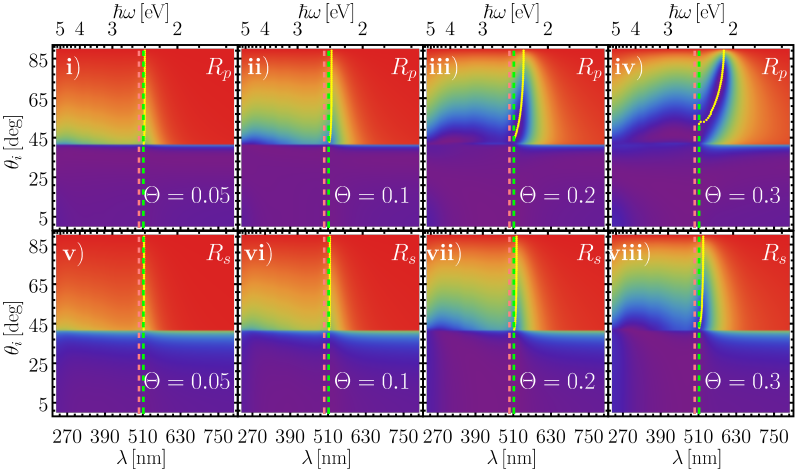
\includegraphics[width = .75\linewidth]{2-Resultados/figs/6-AuThetaVar/0-2D_Grid}%
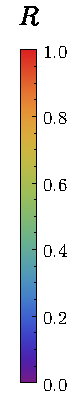
\includegraphics[scale=.85, trim={00 -5 00 00}, clip]{2-Resultados/figs/0-RBar_v}\vspace*{-.5em}
	\caption{Gráficas de reflectancia de una monocapa de NPs esféricas de oro de radio $a=30$ nm en configuración ATR como función del ángulo de incidencia $\theta_i$ y de la longitud de onda $\lambda$ (escala inferior), así como de la energía del haz incidente en unidades de $\hbar\omega$ (escala superior).  Las gráficas   en el renglón superior [$\mathbf{i)-v)}$] muestran los resultados para  polarización \emph{p} y las del renglón inferior  [$\mathbf{vi)-x)}$]  para polarización  \emph{s}, donde se consideraron los valores de fracción de cubierta $\Theta = 0.05,\,0.1,\,0.2$ y $0.3$.  Las líneas verticales punteadas verdes y rosas corresponden a las SP-SPRs dipolar en $\lambda=512$ nm y  cuadrupolar en $\lambda=498$, respectivamente.  Los puntos amarillos corresponden a los mínimos en $R$ para ángulos mayores a $\theta_c\approx 41^\circ$ y longitudes de onda mayores a la SP-SPRs dipolar.
}	\label{fig:Au-R-Theta}	
	\end{figure}	

A diferencia de los cálculos de la reflectacia de una monocapa de NPs  con una función dieléctrica tipo Drude analizada en la sección \ref{ssection:DrudeATR}, en donde sólo se presentaron excitaciones al rededor de las SP-SPRs y el modo colectivo a longitudes de onda mayores a las de las SP-SPRs, los cálculos de la monocapa de NPs de de oro muestran excitaciones a valores de $\lambda$ menores a las de las SP-SPRs (líneas verticales punteadas), las cuales corresponden a excitaciones no plasmónicas, es decir, a contribuciones de transiciones de electrones ligados. Sin embargo, dado que el modo colectivo se excita a energías menores a las de las transiciones interbanda, su contribución no afecta a la excitación colectiva y ésta aún es apreciable, como se observa en las gráficas \textbf{iii), iv), vii)} y \textbf{viii)} de la Fig. \ref{fig:Au-R-Theta}. El modo colectivo, es apreciable para las fracciones de cubierta empleadas de mayor valor ($\Theta = 0.2, 0.3$) y, como sucedió para el análisis con una función dieléctrica tipo Drude, el modo colectivo se aprecia más para polarización \emph{p}, además de traslaparse con la SP-SPRs dipolar.

La reflectancia de una monocapa de NPs con las mismas características que las de la Fig. \ref{fig:Au-R-Theta} pero con NP esféricas de plata de radio $a=30$ nm, se grafica en la Fig. \ref{fig:Ag-R-Theta}, en donde la SP-SPR dipolar corresponde a la línea vertical verde en $\lambda=368$ nm y la cuadrupolar, a la líneas vertical rosa en $\lambda=348$ nm. Al igual que para la monocapa de NPs de oro, se aprecian excitaciones no plasmónicas en valores de $\lambda$ menores a la de las SP-SPRs sin embargo, para la plata estas excitaciones están separadas de las plasmónicas, como se observa por la presencia de la región roja, al rededor de los $300$ nm,  en donde $R\approx 1$. De la misma forma, es apreciable en las gráficas de la Fig. \ref{fig:Ag-R-Theta} el modo colectivo que, para algunos casos, también se separa de la SP-SPRs permitiendo observar ambas.

\begin{figure}[h!]\centering
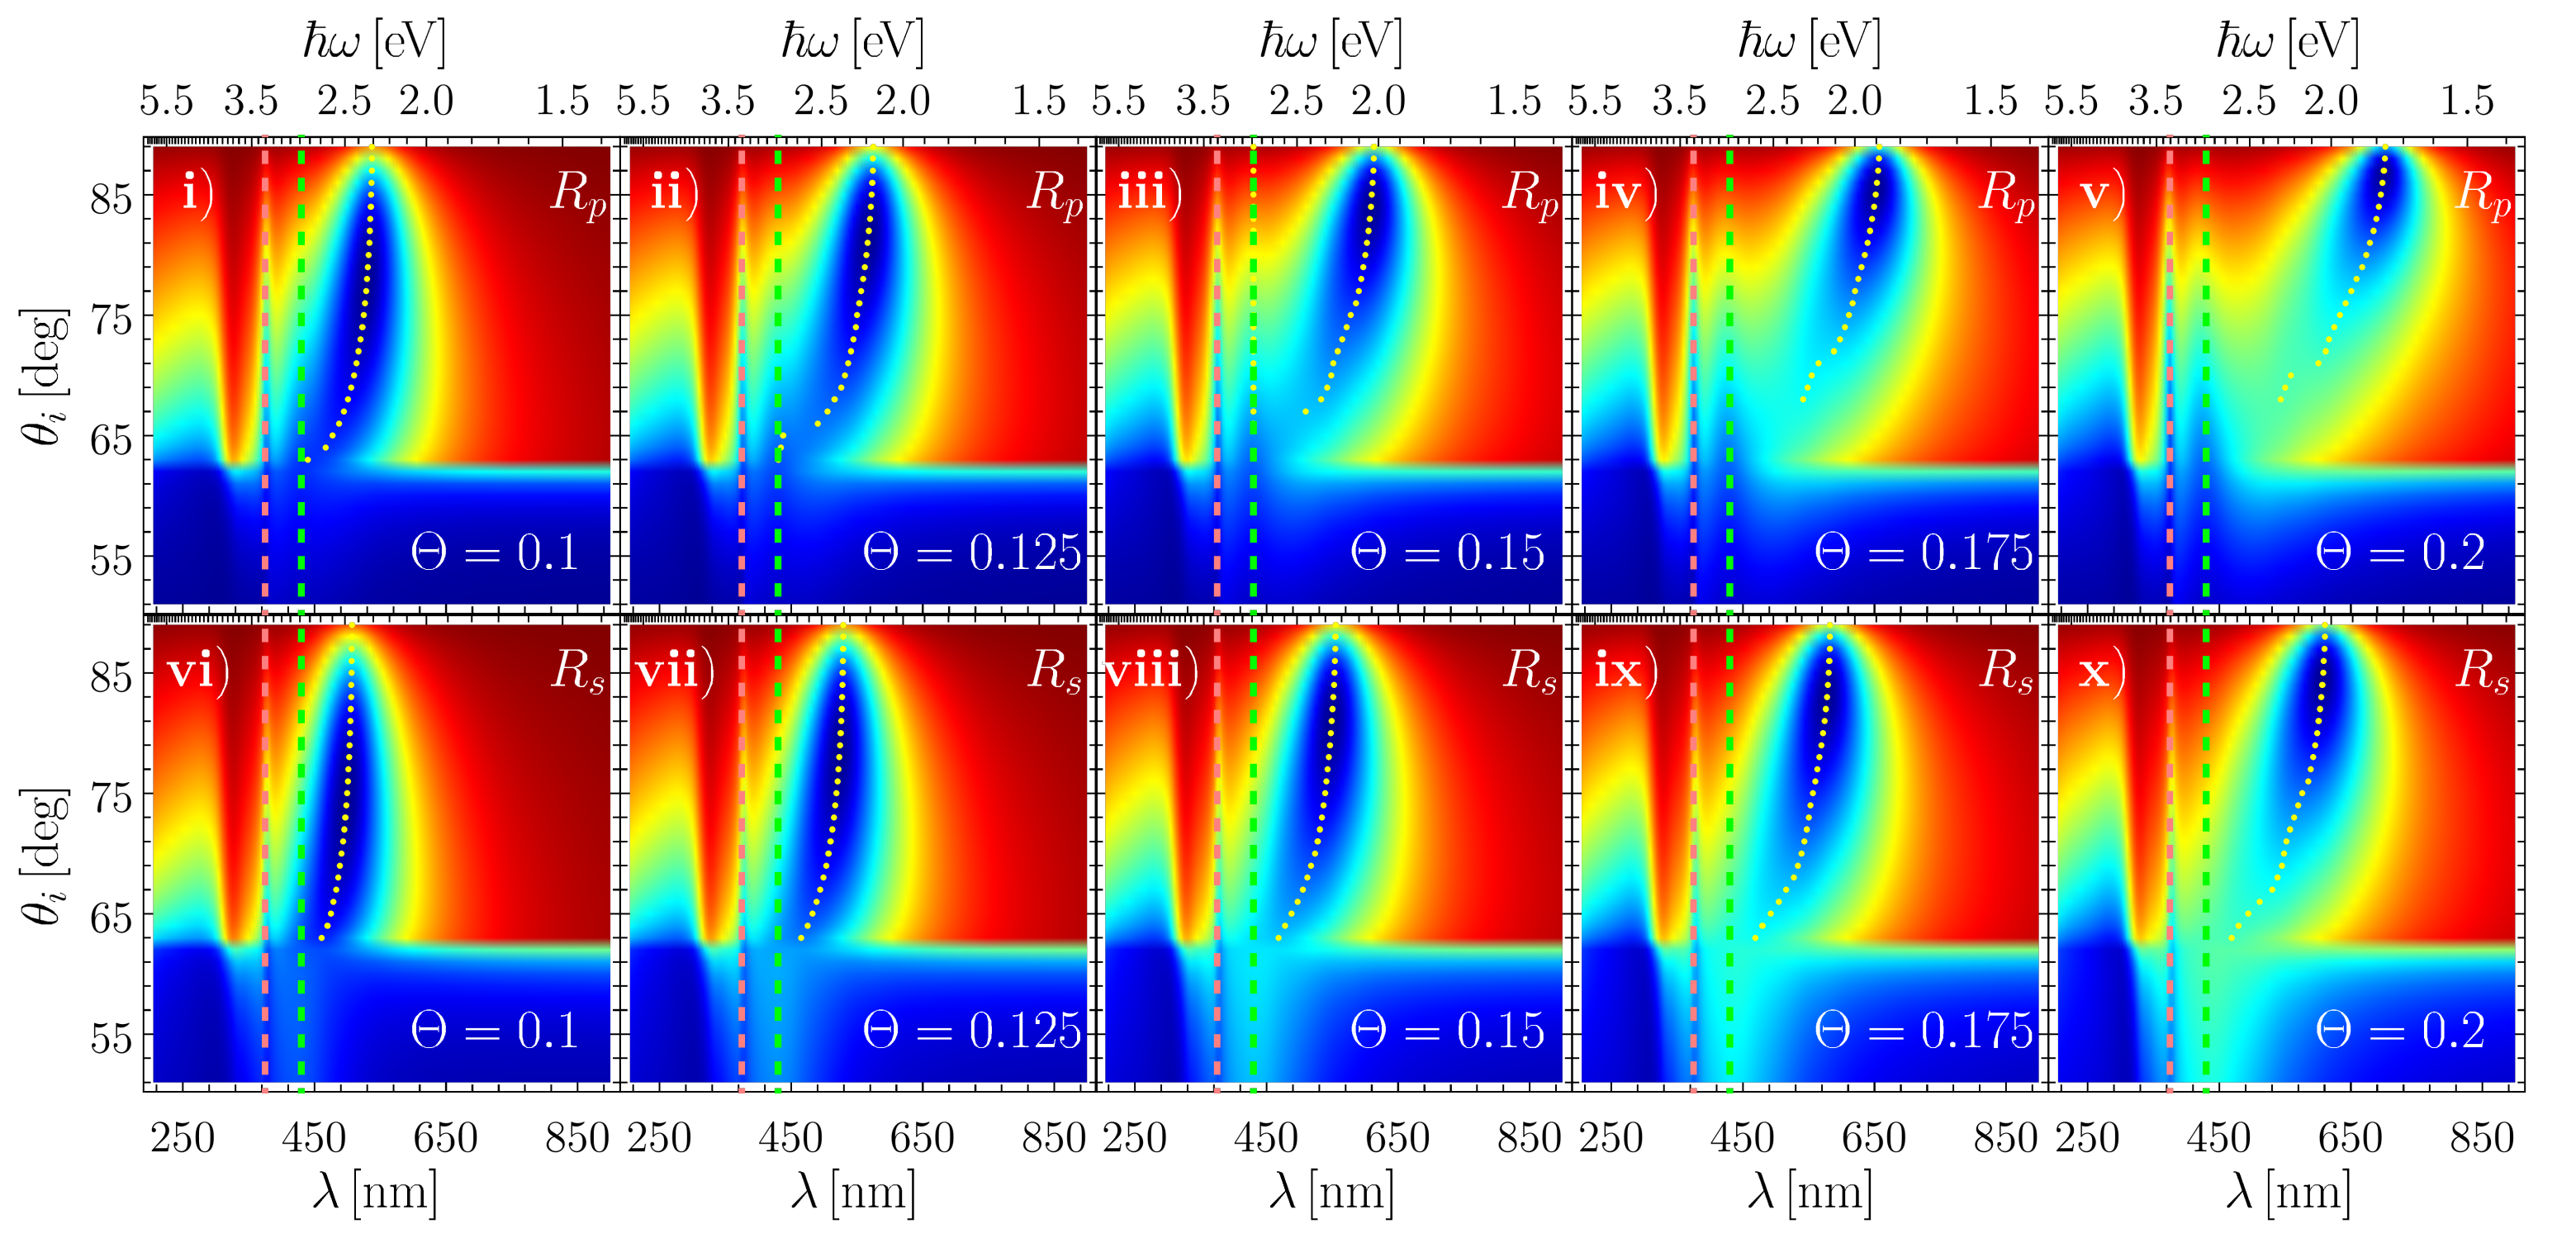
\includegraphics[width = .75\linewidth]{2-Resultados/figs/7-AgThetaVar/0-2D_Grid}%
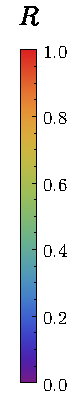
\includegraphics[scale=.85, trim={00 -5 00 00}, clip]{2-Resultados/figs/0-RBar_v}\vspace*{-.5em}
	\caption{Gráficas de reflectancia de una monocapa de NPs esféricas de plata de radio $a=30$ nm en configuración ATR como función del ángulo de incidencia $\theta_i$ y de la longitud de onda $\lambda$ (escala inferior), así como de la energía del haz incidente en unidades de $\hbar\omega$ (escala superior).  Las gráficas   en el renglón superior [$\mathbf{i)-v)}$] muestran los resultados para  polarización \emph{p} y las del renglón inferior  [$\mathbf{vi)-x)}$]  para polarización  \emph{s}, donde se consideraron los valores de fracción de cubierta $\Theta = 0.05,\,0.1,\,0.2$ y $0.3$.  Las líneas verticales punteadas verdes y rosas corresponden a las SP-SPRs dipolar en $\lambda=368$ nm y  cuadrupolar en $\lambda=348$, respectivamente.  Los puntos amarillos corresponden a los mínimos en $R$ para ángulos mayores a $\theta_c\approx 41^\circ$ y longitudes de onda mayores a la SP-SPRs dipolar.
}	\label{fig:Ag-R-Theta}	
	\end{figure}	

El modo colectivo, al igual que con la monocapa de NPS de oro, es apreciable al emplear plata, como se observa en las gráficas \textbf{ii) -- iv), vii)} y \textbf{viii)}, siendo la polarización \emph{p} (gráficas del renglón superior de la Fig. \ref{fig:Ag-R-Theta}) en donde el modo colectivo (puntos amarillos) es más apreciable. Igualmente, las SP-SPRs se distinguen de la excitación colectiva para los valores de $\Theta\geq 0.1$  para polarización \emph{p}, mientras que para polarización \emph{s} las excitaciones de partícula individual se traslapan con el modo colectivo para todos los casos de $\Theta=0.2$ y $0.3$. Para $\Theta = 0.05$ y $0.1$ y polarización \emph{s}, el modo colectivo no es apreciable, como tampoco lo es para $\Theta=0.05$ en polarización \emph{p}.

Dado que el modo colectivo se presenta para monocapas de NPs tanto de oro como de plata, ambos materiales pueden emplearse en el biosensado. Para analizar las diferencias entre la respuesta EM de una monocapa de NPs esféricas de oro y plata, se grafican, en la Fig. \ref{fig:AuAg-Cuts}, cortes a $\theta_i = 65^\circ$ de la reflectancia de la Fig. \ref{fig:Au-R-Theta}, donde se emplean NPs de oro, y de la Fig. \ref{fig:Ag-R-Theta}, donde se consideran NPs de plata. En las Figs. \ref{sfig:Au-cutp} y \ref{sfig:Au-cuts} se grafica la reflectancia para una monocapa de NPs de oro al incidir una onda plana con polarización \emph{p} y \emph{s}, respectivamente, mientras que en las Figs. \ref{sfig:Ag-cutp} y \ref{sfig:Ag-cuts} se grafica la reflectancia para una monocapa de NPs de plata para polarización \emph{p} y \emph{s}, respectivamente.

\begin{figure}[h!]\centering\hspace*{-1.5em}
	\begin{subfigure}{.01\linewidth}\caption{}\label{sfig:Au-cutp}\vspace{4.5cm}\end{subfigure}
	\begin{subfigure}{.45\linewidth}\hspace*{-1.5em}
	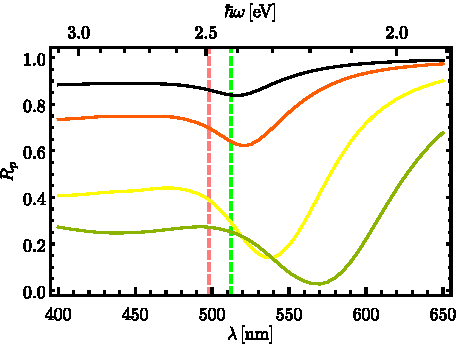
\includegraphics[scale=1]{2-Resultados/figs/6-AuThetaVar/cut_angle_65_p.pdf}\end{subfigure}
	\begin{subfigure}{.01\linewidth}\caption{}\label{sfig:Au-cuts}\vspace{4.5cm}\end{subfigure}\hspace*{-1.em}
	\begin{subfigure}{.45\linewidth}\centering
	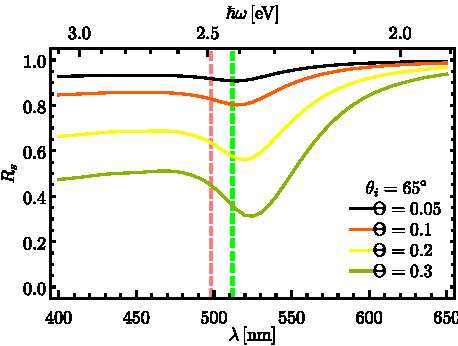
\includegraphics[scale=1 ]{2-Resultados/figs/6-AuThetaVar/cut_angle_65_s.pdf}\end{subfigure}\vspace*{0em}\\
	\hspace*{-1.5em}
	\begin{subfigure}{.01\linewidth}\caption{}\label{sfig:Ag-cutp}\vspace{4.5cm}\end{subfigure}
	\begin{subfigure}{.45\linewidth}\hspace*{-1.5em}
	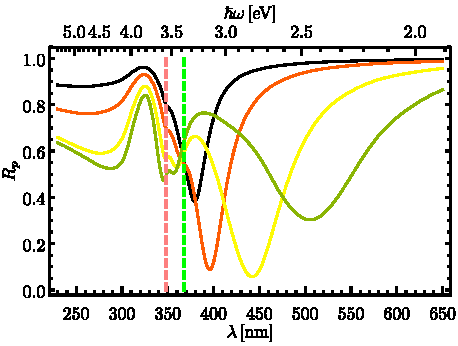
\includegraphics[scale=1]{2-Resultados/figs/7-AgThetaVar/cut_angle_65_p.pdf}\end{subfigure}
	\begin{subfigure}{.01\linewidth}\caption{}\label{sfig:Ag-cuts}\vspace{4.5cm}\end{subfigure}\hspace*{-1.em}
	\begin{subfigure}{.45\linewidth}\centering
	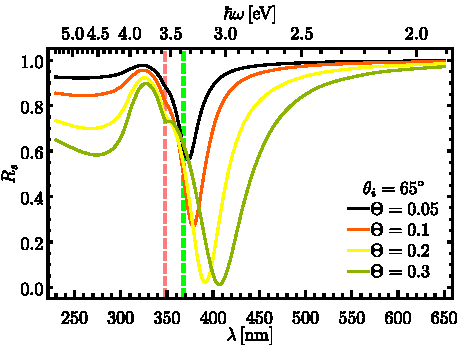
\includegraphics[scale=1 ]{2-Resultados/figs/7-AgThetaVar/cut_angle_65_s.pdf}\end{subfigure}\vspace*{-.5em}
	\caption{Cortes a $\theta_i = 65^\circ$ de las gráficas de reflectancia de una monocapa en configuración ATR (Fig. \ref{fig:R-RVar}) de NPs esféricas de fracción de cubierta $\Theta = 0.3$ en polarización \textbf{a)} \emph{p} y \textbf{b)} \emph{s} como función de la longitud de onda $\lambda$ (escala inferior) y de la energía $\hbar\omega$ (escala superior). Los parámetros de la función dieléctrica tipo Drude para las NPs son $\omega_p = 4.3$ eV y $\gamma = 0.15$ eV y las fracciones de cubierta consideradas fueron $a$: $3$ nm, $5$ nm, $10$ nm y $20$ nm. La SP-SPR dipolar para los tamaños de partículas utilizadas corresponde la región verde entre $500$ nm y $512$ nm, mientras que la cuadrupolar corresponde a la región rosa entre $456$ nm y $462$ nm.}\label{fig:AuAg-Cuts}
	\end{figure}	

Los resultados para la monocapa de NPs de oro de $a=30$ nm presentan una menor reflectancia en el intervalo de $500$ nm$<\lambda<650$ nm para ambas polarizaciones conforme aumenta la fracción de cubierta $\Theta$. Asimismo, se presenta sólo un mínimo en los cálculos de la reflectancia para ambas polarizaciones que se corre al rojo, además de ser más pronunciado, conforme aumenta el valor de $\Theta$. Como se observó en la Fig. \ref{fig:Au-R-Theta}, las SP-SPRs no son apreciables para ninguna polarización, excepto en el caso de $\Theta =0.05$, donde el efecto de partícula individual es válido y por tanto la SP-SPR dipolar coincide con la única excitación presente en $\lambda = 512$ nm. Al comparar las Figs. \ref{sfig:Au-cutp} y \ref{sfig:Au-cuts} se corrobora que el corrimiento al rojo de la única excitación apreciable  es mayor para polarización \emph{p}, al igual que el decrecimiento en la reflectancia, como se observa en el caso de $\Theta=0.2$, donde para polarización \emph{p} el mínimo en reflectancia se localiza a $\lambda\approx  540$ nm  y $R \approx 0.2$, mientras que en polarización \emph{s}, $\lambda\approx 520$ nm y $R\approx 0.5$.

Cuando se consideran NPs de plata de $a=30$ nm para la monocapa, se presenta un máximo en la reflectancia tanto para polarización \emph{p} [Fig. \ref{sfig:Ag-cutp}] como para \emph{s} [Fig. \ref{sfig:Ag-cuts}]  a $\lambda \approx 330$ nm, valor de la longitud de onda que separa las excitaciones no plasmónicas ($\lambda<330$ nm) de las plasmónicas. Dentro de las SP-SPRs apreciables en la reflectancia de la monocapa se encuentra la resonancia cuadrupolar a $\lambda = 348$ nm (línea vertical rosa) para todos valores de $\Theta$ analizados y para ambas polarizaciones. En la Fig. \ref{sfig:Ag-cutp}, se aprecia en el intervalo $348$ nm$<\lambda<368$ nm y para $\Theta\geq 0.1$ un mínimo en $R_p$ que se corre al azul a valores de $\Theta$ mayores, por lo que puede ser un corrimiento al azul de la SP-SPR dipolar dado que la distancia promedio entre las NPs disminuye. El caso de $\Theta =0.05$, en polarización \emph{p}, no presenta ningún mínimo en la reflectancia a valores de $\lambda$ entre los de las SP-SPRs dipolar y cuadrupolar mas presenta un mínimo a $\lambda\approx 380$ nm, es decir, a longitudes de onda mayores, en donde $R_p\approx 0.4$. Para los casos de $\Theta = 0.1$ y $0.2$, también se aprecia un mínimo a longitudes de onda mayores que la de la SP-SPR dipolar y éste se corre al rojo conforme aumenta el valor de la fracción de cubierta, al igual que disminuye el valor de $R$, por ejemplo, para  $\Theta = 0.2$ el mínimo en $R_p$ se presenta a $\lambda \approx 440$ nm y $R_p \approx 0.05$. Esta tendencia sólo no se presenta para el caso de $\Theta = 0.3$ donde el valor de la reflectancia evaluada a la longitud de onda de la excitación ($\lambda \approx 510$ nm) aumenta respecto al del caso de $\Theta = 0.02$. Al considerar la polarización \emph{s} [Fig. \ref{sfig:Ag-cuts}], se aprecia únicamente la excitación a valores de $\lambda$ mayores a la de la SP-SPRs dipolar y ésta se corre al rojo y disminuye el valor de la reflectancia en estas longitudes de onda al crecer el valor de $\Theta$.

Las respuestas EM de una monocapa de NPs  de oro y una de plata presentan el comportamiento del modo colectivo a longitudes de onda mayores a las de la SP-SPRs dipolar (línea vertical verde en la Fig. \ref{fig:AuAg-Cuts}) sin embargo, las características de esta excitación son distintas para cada uno de los materiales. Si bien para ambos materiales la resonancia colectiva se corre al rojo conforme aumenta la fracción de cubierta, para el oro ésta se localiza en el intervalo $512$ nm$<\lambda<570$ nm en polarización \emph{p} [ver Fig. \ref{sfig:Au-cutp}] y  en polarización \emph{s} [ver Fig. \ref{sfig:Au-cuts}] en el intervalo  $512$ nm$<\lambda<530$ nm, es decir, que se encuentran dentro del espectro visible. Por otro lado, para la monocapa de NPs de plata, el modo colectivo se localiza para $\Theta = 0.05$ y $0.1$ en el ultravioleta para ambas polarizaciones; al aumentar $\Theta$, el modo colectivo se presenta a longitudes de onda entre $440$ nm y $520$ nm para polarización \emph{p} [ver Fig. \ref{sfig:Ag-cutp}] y entre $380$ nm y $410$ nm para polarización \emph{s} [ver Fig. \ref{sfig:Ag-cuts}]. Adicional al intervalo donde ocurre el modo colectivo, el valor de la reflectancia a los longitudes de onda de la excitación son menores para la monocapa de NPs de plata que para la de NPs de oro, por ejemplo, para la plata la reflectancia en los valores de $\lambda$ del modo colectivo es menor a $0.6$ para todos los casos como se observa en las Figs. \ref{sfig:Ag-cutp} y \ref{sfig:Ag-cuts}, mientras que para el oro $R<0.6$ sólo para $\Theta\geq 0.2$ [ver Figs. \ref{sfig:Ag-cutp} y \ref{sfig:Ag-cuts}]. Dado que en análisis de la reflectancia para una monocapa de NPs con una función dieléctrica tipo Drude mostró que es posible sintonizar la respuesta colectiva, así como disminuir el valor de la reflectancia a las longitudes de onda de la excitación colectiva, al modificar el radio de las NPs, por lo que se analiza el comportamiento de las monocapas de NPs de oro y plata, al variar el radio $a$ de éstas y considerando $\Theta = 0.2$, valor en el que el cociente de la distancia promedio entre NPs $\langle d \rangle$ y el radio de las NPs es $\langle d \rangle / a = 1.96 $, por lo que el límite diluido está garantizado.

\begin{figure}[b!]\centering
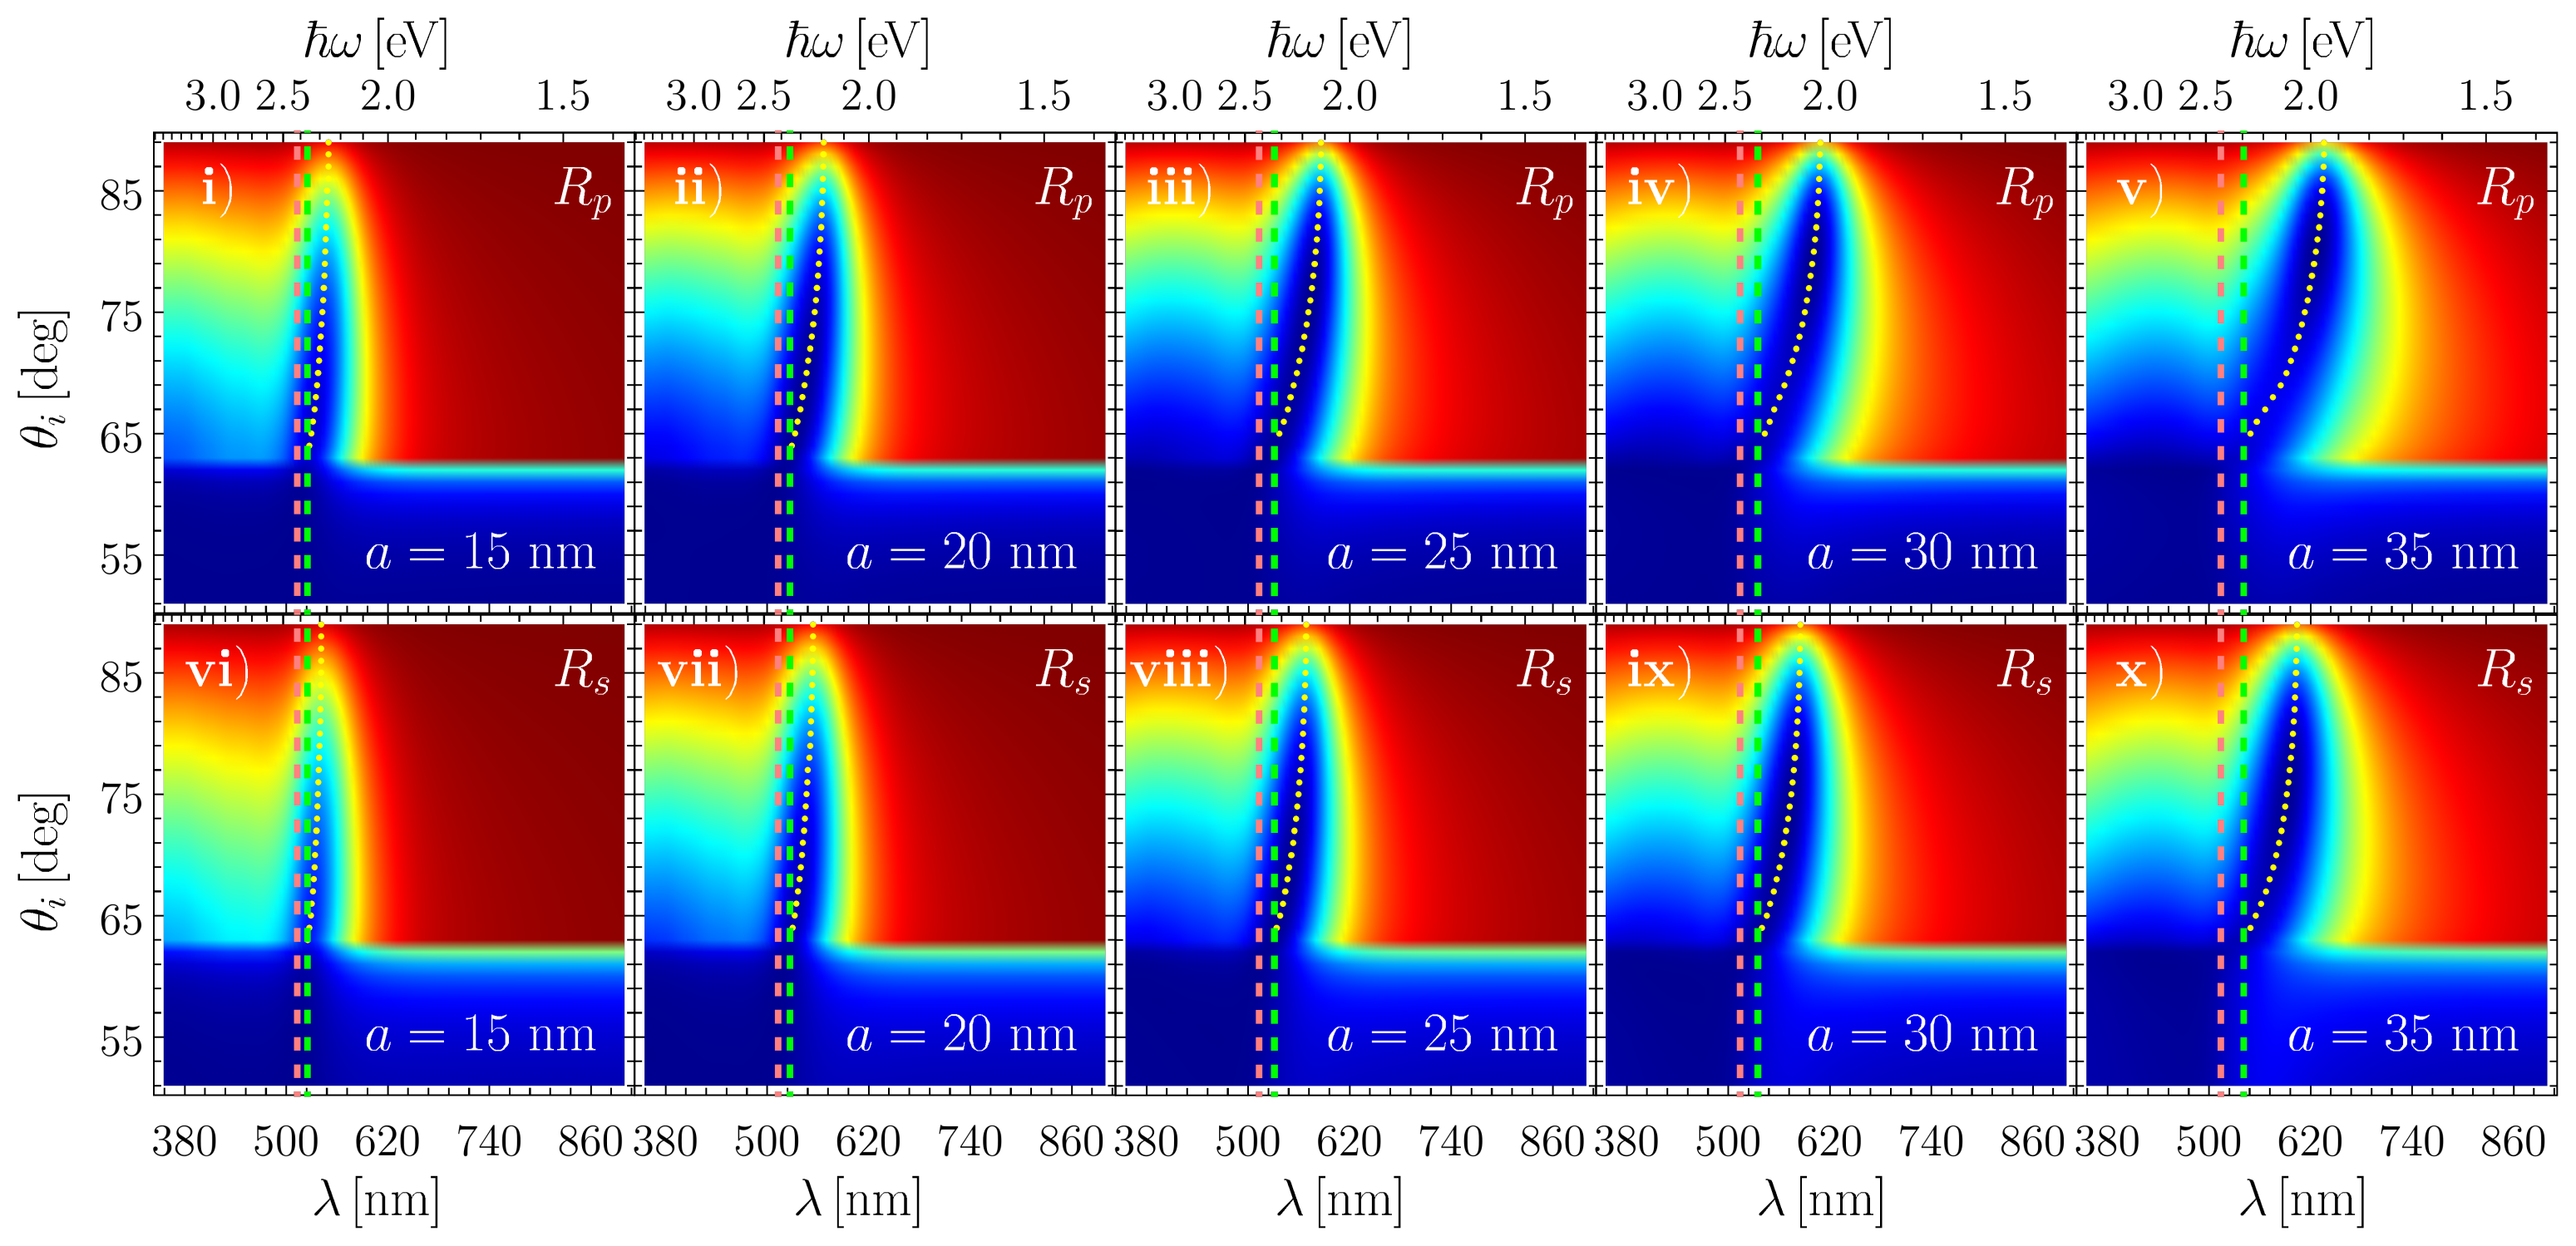
\includegraphics[width = .75\linewidth]{2-Resultados/figs/8-AurVar/0-2D_Grid}%
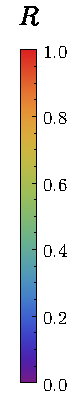
\includegraphics[scale=.85, trim={00 -5 00 00}, clip]{2-Resultados/figs/0-RBar_v}\vspace*{-.5em}
	\caption{Gráficas de reflectancia de una monocapa en configuración ATR como función del ángulo de incidencia $\theta_i$ y de la longitud de onda $\lambda$ (escala inferior), así como de la energía del haz incidente en unidades de $\hbar\omega$ (escala superior), para una función dieléctrica tipo Drude con $\omega_p=4.3$ eV  y  $\gamma=0. 15$ eV.  Las gráficas   en el renglón superior [$\mathbf{i)-v)}$] muestran los resultados para  polarización \emph{p} y las del renglón inferior  [$\mathbf{vi)-x)}$]  para polarización  \emph{s}, donde se consideró una fracción de cubierta $\Theta = 0.3$ y  NPs de radio  $a$: $3$ nm, $5$ nm, $10$ nm y $20$ nm.  Las líneas verticales punteadas verdes y rosas corresponden a las SP-SPRs dipolar y  cuadrupolar, respectivamente.  Los puntos amarillos corresponden a los mínimos en $R$ para ángulos mayores a $\theta_c\approx 41^\circ$ y longitudes de onda mayores a la SP-SPRs dipolar.
}	\label{fig:Au-R-Rad}	
	\end{figure}	

En la Fig. \ref{fig:Au-R-Rad} se grafica la reflectancia para una monocapa de NPs de oro con una fracción de cubierta $\Theta = 0.2$, inmersa en aire ($n_m = 1$) y soportada por un sustrato con $n_s = 1.5$, como función del ángulo de incidencia $\theta_i$, de la longitud de onda $\lambda$ (escala inferior) y de la energía en unidades de $\hbar\omega$ (escala superior). Tanto para la monocapa de NPs de oro, como las de plata, en las gráficas \textbf{i) -- iv)} se presentan los casos para polarización \emph{p} y en las gráficas \textbf{v) -- viii)} para polarización \emph{s}, al considerar NPs con radios $a= 20$ nm, $30$ nm, $40$ nm y $50$ nm. Las líneas verticales punteadas corresponden a las longitudes de onda donde se excitan las SP-SPRs dipolares (verdes) y cuadrupolares (rosas); para $a= 20$ nm la excitación dipolar se presenta a $\lambda \approx 510$ mientras que para $a = 30$ nm, $40$ nm y $50$ nm a $512$ nm, $516$ nm y $521$ nm, respectivamente; la excitación cuadrupolar para todos los radios se presenta a $\lambda\approx 498$ nm. Los puntos amarillos corresponden al modo colectivo.

Para la monocapa de NPs de oro, la respuesta EM en el régimen de las excitaciones no plasmónicas difiere al variar el radio $a$ de las NPs que al variar la fracción de cubierta $\Theta$. Al variar el radio de las NPs, manteniendo un valor de $\Theta = 0.2$, la radiación EM reflejada a valores de $\lambda$ menores a los de las SP-SPRs es mayor al aumentar el ángulo de incidencia $\theta_i$, como se muestra en la Fig. \ref{fig:Au-R-Rad}. En cambio cuando se varió el valor de $\Theta$, manteniendo un radio constante de $a=30$ nm [Fig. \ref{fig:Au-R-Theta}], la luz se reflejó en menor medida al aumentar $\theta_i$. Este comportamiento puede permitir obtener un mayor contraste entre la reflectancia evaluada en los valores de $\lambda$ del modo colectivo y el resto de los valores de $\lambda$. El comportamiento de las SP-SPRs en la respuesta EM de la monocapa de NPs de oro es equivalente al caso de la variación de $\Theta$. Para el oro,  las SP-SPRs se traslapan con la única excitación apreciable: para polarización \emph{s} considerando $a= 20$ nm, gráfica \textbf{v)}, y $a= 30$ nm, \textbf{vi)}, las SP-SPRs dipolar coincide con la excitación presente. Para los valores de $a=40$ nm y $50$ nm en polarización \emph{s}, gráficas \textbf{vii)} y \textbf{viii)}, así como para todos los radios considerados en polarización \emph{p}, gráficas \textbf{i) -- iv)}

\begin{figure}[b!]\centering
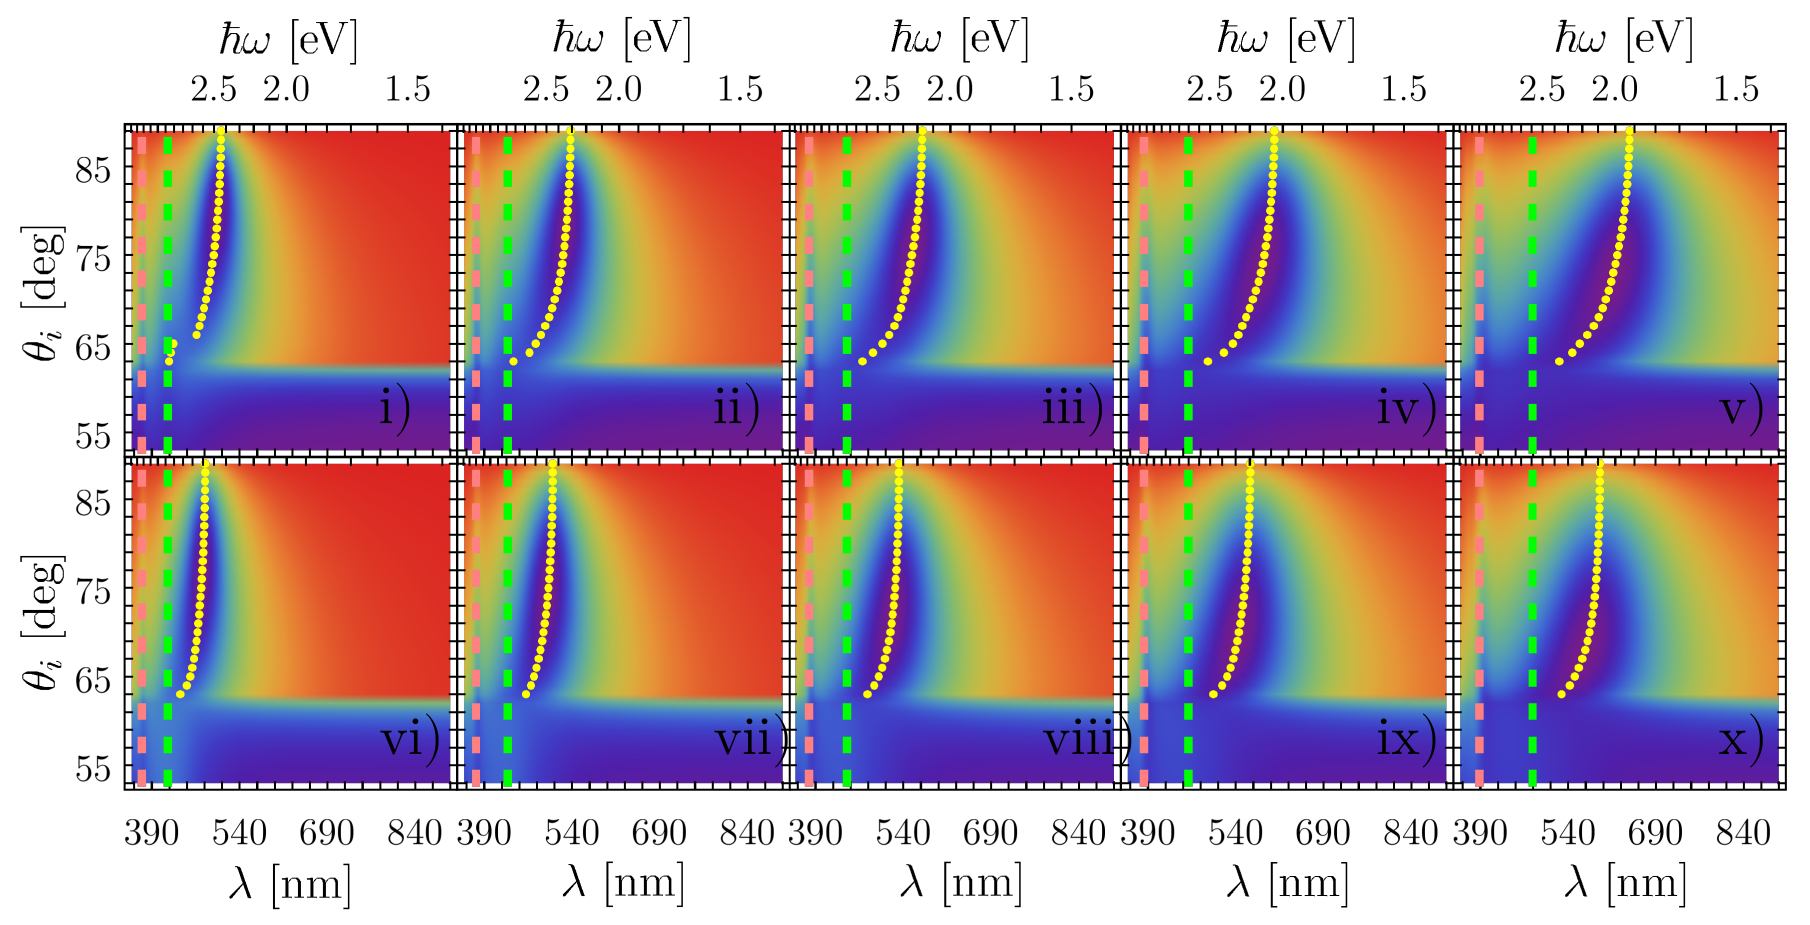
\includegraphics[width = .75\linewidth]{2-Resultados/figs/9-AgrVar/0-2D_Grid}%
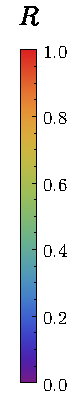
\includegraphics[scale=.85, trim={00 -5 00 00}, clip]{2-Resultados/figs/0-RBar_v}\vspace*{-.5em}
	\caption{Gráficas de reflectancia de una monocapa en configuración ATR como función del ángulo de incidencia $\theta_i$ y de la longitud de onda $\lambda$ (escala inferior), así como de la energía del haz incidente en unidades de $\hbar\omega$ (escala superior), para una función dieléctrica tipo Drude con $\omega_p=4.3$ eV  y  $\gamma=0. 15$ eV.  Las gráficas   en el renglón superior [$\mathbf{i)-v)}$] muestran los resultados para  polarización \emph{p} y las del renglón inferior  [$\mathbf{vi)-x)}$]  para polarización  \emph{s}, donde se consideró una fracción de cubierta $\Theta = 0.3$ y  NPs de radio  $a$: $3$ nm, $5$ nm, $10$ nm y $20$ nm.  Las líneas verticales punteadas verdes y rosas corresponden a las SP-SPRs dipolar y  cuadrupolar, respectivamente.  Los puntos amarillos corresponden a los mínimos en $R$ para ángulos mayores a $\theta_c\approx 41^\circ$ y longitudes de onda mayores a la SP-SPRs dipolar.
}	\label{fig:Ag-R-Rad}	
	\end{figure}	

Los cálculos de la reflectancia de una monocapa de NPs de plata con $\Theta= 0.2$ se grafican en la Fig. \ref{fig:Ag-R-Rad} como función de $\theta_i$, $\lambda$ y $\hbar\omega$. Se consideró un sustrato con índice de refracción $n_s=1.5$ y una matriz con $n_m=1.5$. En la Fig. \ref{fig:Ag-R-Rad}, las líneas punteadas verticales verdes corresponden a la SP-SPR dipolar y las rosas a la cuadrupolar; al considerar NPs de plata, las longitudes de onda de la SP-SPR dipolar son $360$ nm, $368$ nm, $379$ nm y $393$ nm, para $a = 20$ nm, $30$ nm, $40$ nm y $50$ nm, respectivamente; mientras que  la SP-SPR cuadrupolar se excita a $347$ nm, $348$ nm, $350$ nm y $353$ nm para NPs de radio $a = 20$ nm, $30$ nm, $40$ nm y $50$ nm, respectivamente.

La reflectancia de una monocapa de NPs de plata (Fig. \ref{fig:Ag-R-Rad}) para $\lambda\approx 300$ nm es cercana a la unidad para todos los radios $a$ considerados, comportamiento que también se observó en la Fig. \ref{fig:Ag-R-Theta} cuando se varió $\Theta$. Esta característica, presente sólo para la plata, puede emplearse para la caracterización del material empleado para las NPs de una monocapa. Para las longitudes de onda de las SP-SPRs, las excitaciones cuadrupolares (líneas verticales punteadas rosas) son más apreciables que las dipolares, para $\theta_i>\theta_c\approx 41^\circ$. Finalmente, respecto al  modo colectivo (puntos amarillos en la Fig. \ref{fig:Ag-R-Rad}) su comportamiento es semejante al observado para el oro en la Fig. \ref{fig:Au-R-Rad}: al aumentar el radio de las NPs, el modo colectivo es más apreciable y se corre hacia el rojo, efecto que se aprecia más para polarización \emph{p} que para \emph{s}.

Para comparar los resultados de la reflectancia al emplear la función dieléctrica de del oro y de la plata para las NPs, se grafican en la Fig. \ref{fig:AuAg-Cuts-Rad} cortes a $\theta_i = 65^\circ$ de la relfectancia $R$ de las Figs. \ref{fig:Au-R-Rad} y \ref{fig:Ag-R-Rad}. Las Figs. \ref{sfig:Au-cutp-Rad} y \ref{sfig:Au-cuts-Rad} son las gráficas de la reflectancia de una monocapa de NPs de oro con una onda plana incidiendo con polarización \emph{p} y \emph{s}, respectivamente, mientras que las Figs.  \ref{sfig:Ag-cutp-Rad} y\ref{sfig:Ag-cuts-Rad}  corresponden a la relfectancia de una monocapa de NPs de plata para polarización \emph{p} y \emph{s}, respectivamente. En todas las gráficas de la Fig. \ref{fig:AuAg-Cuts-Rad} la región sombreada verde corresponde al intervalo en $\lambda$ de las SP-SPRs para los radios $a=20$ nm, $30$ nm, $40$ nm y $50$ nm tanto para la excitación dipolar (región verde), como la cuadrupolar (rosa). 

\begin{figure}[h!]\centering\hspace*{-1.5em}
	\begin{subfigure}{.01\linewidth}\caption{}\label{sfig:Au-cutp-Rad}\vspace{4.5cm}\end{subfigure}
	\begin{subfigure}{.45\linewidth}\hspace*{-1.5em}
	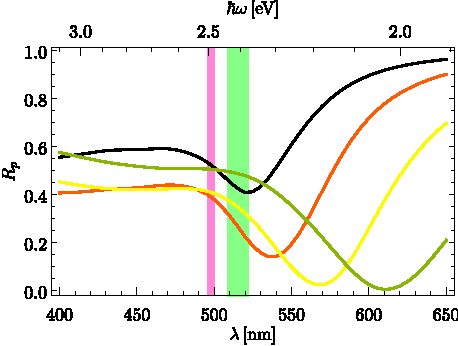
\includegraphics[scale=1]{2-Resultados/figs/8-AurVar/cut_angle_65_p.pdf}\end{subfigure}
	\begin{subfigure}{.01\linewidth}\caption{}\label{sfig:Au-cuts-Rad}\vspace{4.5cm}\end{subfigure}\hspace*{-1.em}
	\begin{subfigure}{.45\linewidth}\centering
	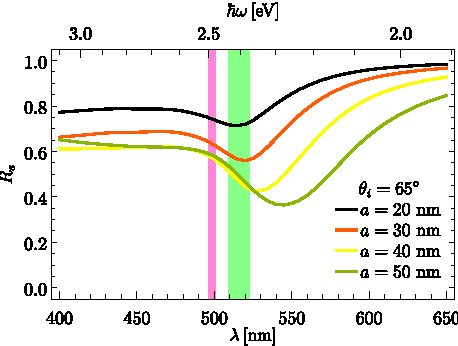
\includegraphics[scale=1 ]{2-Resultados/figs/8-AurVar/cut_angle_65_s.pdf}\end{subfigure}\vspace*{-0em}\\
	\hspace*{-1.5em}
	\begin{subfigure}{.01\linewidth}\caption{}\label{sfig:Ag-cutp-Rad}\vspace{4.5cm}\end{subfigure}
	\begin{subfigure}{.45\linewidth}\hspace*{-1.5em}
	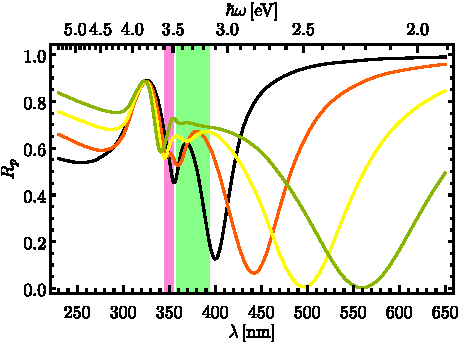
\includegraphics[scale=1]{2-Resultados/figs/9-AgrVar/cut_angle_65_p.pdf}\end{subfigure}
	\begin{subfigure}{.01\linewidth}\caption{}\label{sfig:Ag-cuts-Rad}\vspace{4.5cm}\end{subfigure}\hspace*{-1.em}
	\begin{subfigure}{.45\linewidth}\centering
	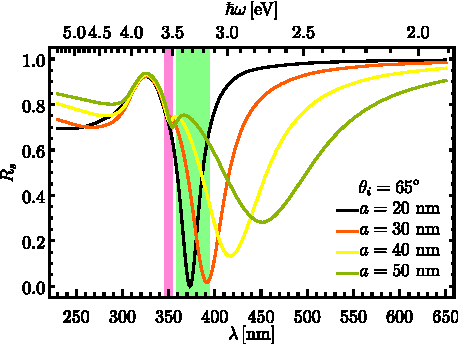
\includegraphics[scale=1 ]{2-Resultados/figs/9-AgrVar/cut_angle_65_s.pdf}\end{subfigure}\vspace*{-.5em}
	\caption{Cortes a $\theta_i = 65^\circ$ de las gráficas de reflectancia de una monocapa en configuración ATR (Fig. \ref{fig:R-RVar}) de NPs esféricas de fracción de cubierta $\Theta = 0.3$ en polarización \textbf{a)} \emph{p} y \textbf{b)} \emph{s} como función de la longitud de onda $\lambda$ (escala inferior) y de la energía $\hbar\omega$ (escala superior). Los parámetros de la función dieléctrica tipo Drude para las NPs son $\omega_p = 4.3$ eV y $\gamma = 0.15$ eV y las fracciones de cubierta consideradas fueron $a$: $3$ nm, $5$ nm, $10$ nm y $20$ nm. La SP-SPR dipolar para los tamaños de partículas utilizadas corresponde la región verde entre $500$ nm y $512$ nm, mientras que la cuadrupolar corresponde a la región rosa entre $456$ nm y $462$ nm.}\label{fig:AuAg-Cuts-Rad}
	\end{figure}	

Para el caso de una monocapa de NPs de oro [Figs. \ref{sfig:Au-cutp-Rad} y \ref{sfig:Au-cuts-Rad}], se presenta un mínimo en la reflectancia $R$ a longitudes de onda mayores a las de las SP-SPRs por lo que se identifica como el modo colectivo. Reproduciendo la tendencia observada para monocapas de NPs con una función dieléctrica tipo Drude, al aumentar el tamaño de las NPs, la excitación colectiva sufre un corrimiento al rojo en ambas polarizaciones: para polarización \emph{p} el modo colectivo se excita en el intervalo entre $520$ nm y $620$ nm y para polarización \emph{s} entre $510$ nm y $550$ nm. Al comparar el corrimiento al rojo al variar el radio de las NPs, con $\Theta=0.2$, y al variar la fracción de cubierta, con $a=30$ nm [ver Fig. \ref{fig:Au-R-Theta}], se observa que el corrimiento al rojo es mayor al considerar NPs más grandes que al considerar mayores fracciones de cubierta. De igual forma, los valores de la reflectancia a los valores de $\lambda$ del modo colectivo cumple con que  $R<0.2$ para $a\geq 30$ nm en polarización \emph{p} [ver Fig. \ref{sfig:Au-cutp-Rad}] y  para polarización \emph{s}  [ver Fig. \ref{sfig:Au-cuts-Rad}] $0.4<R<0.8$, que son valores menores a los observados en la variación de $\Theta$ en la Fig. \ref{fig:AuAg-Cuts}.

Respecto a la respuesta EM de una monocapa de NPs de plata, se observa en las Figs. \ref{sfig:Ag-cutp-Rad} y \ref{sfig:Ag-cuts-Rad} un máximo en la reflectancia en $\lambda \approx 330$ nm, que se apreciaba a distintos valores de $\Theta$ en la Fig. \ref{fig:AuAg-Cuts}. Al considerar el radio de las NPs variable pero la fracción de cubierta constante, se corrobora que el valor de $R_p$ y $R_s$ en $\lambda\approx 330$ nm es constante para un $\Theta$ fijo, por lo que puede emplearse esta longitud de onda para caracterizar la fracción de cubierta de una monocapa de NPs esféricas de plata; en particular para $\Theta=0.2$, $R_p = 0.9$ y $R_s = 0.95$ en $\lambda \approx 330$ nm. Una característica en común con la variación de $\Theta$, es que al aumentar el radio de las NPs de plata aún es apreciable la resonancia cuadrupolar de partícula individual considerando un corrimiento de esta excitación hacia le azul, como se observa en los mínimos en $R_p$ al rededor de la región rosa; en polarización \emph{s} la excitación cuadrupolar sólo es apreciable para $a=40$ nm y $50$ nm. La SP-SPR dipolar es también es apreciable para la polarización \emph{p} en la región de $360$ nm$<\lambda<390$ nm sin embargo, no es apreciable para la polarización \emph{s} dado que se traslapa con la excitación del modo colectivo. La excitación colectiva, al igual que se en caso de las NPs de oro, sufre un corrimiento al rojo mayor al aumentar el radio de las NPs que al aumentar la fracción de cubierta, además de disminuir el valores de $R$ al evaluarlo en la longitud de onda de la excitación colectiva: para polarización \emph{p} el modo colectivo se excita entre $400$ nm y $550$ nm, es decir que se sintoniza en la mitad del espectro visible, además de que para $20$ nm y $30$ nm $R_p<0.2$ y para $40$ nm y $50$ nm $R_p \approx 0$; para polarización \emph{s}, $R_s\leq 0.2$ al excitar el modo colectivo ($370$ nm$<\lambda<460$ nm) para $a\leq 40$ nm y $R_s\approx 0.4$ para $a=50$ nm.



La construcción de un sensor para materia biológica basado en la respuesta EM colectiva de una monocapa de NPs plasmónicas es posible al emplear oro o plata, según los resultado de la reflectancia graficados en la Fig. \ref{fig:AuAg-Cuts}.  En l




